\chapter{Exposé}

\section{Introduction}

The game 'Who Am I' has various names and exists in numerous forms and variations. Each player can represent virtually anything, which increases the difficulty, and the number of players can also vary. A typical version of the game for children is a $4 \times 6$ board that includes only persons. This version is further referred to for a more specific analysis, but a similar ratio is expected for a scaled-up version.

\section{Theoretical Background and State of the Art}
\label{sec:state-of-the-art}

The field of RL has witnessed significant advancements in recent years, particularly in its application to complex decision-making processes. RL algorithms, inspired by behavioral psychology, have demonstrated remarkable capabilities in learning optimal strategies through trial and error interactions with environments. Concurrently, stochastic modelling techniques have long been employed to analyze uncertainty and randomness in various systems. This includes stochastic processes, which offer powerful frameworks for modelling dynamic systems influenced by probabilistic factors. In the context of game theory and decision-making tasks, RL has been successfully applied to games like "Guess Who?", where developing an optimal strategy involves managing uncertainty and making sequential decisions based on partial information. The integration of RL with stochastic approaches presents a promising avenue for addressing challenges such as uncertainty, scalability, and adaptability. Recent research has explored the synergy between RL and stochastic methods in diverse domains, ranging from robotics and game theory to finance and healthcare. By leveraging the strengths of both paradigms, researchers aim to develop more robust and efficient solutions for decision-making tasks in complex and uncertain environments.


\section{Research Question}

The original research question was: What is the optimal number of questions required to accurately identify a specific individual out of a set of 24 persons using reinforcement learning and stochastic modelling techniques? However, feedback from the advisor highlighted that this question has been partially answered by the YouTuber Mark Rober. Therefore, the research question has been refined to focus on analyzing the reinforcement learning strategy in comparison to Mark Rober's optimal strategy and other existing optimal strategies. Additionally, the research will explore how the number of questions required changes when parameters such as the number of persons are varied or when the scope is expanded to include not only persons but also non-person entities. This more specific approach aims to provide deeper insights into the adaptability and scalability of the RL algorithm's strategy under different conditions and contributes to the novelty of the thesis.


\section{Methodology}

The approach is going to be a practical realization, aimed at addressing the research question of how the learned strategy of the RL algorithm compares to stochastic strategies, as well as other existing optimal strategies. The methodology will include the design and implementation of the RL training environment, the selection of appropriate reward functions, and the evaluation metrics used to measure performance. Furthermore, the analysis will extend to examining the number of questions needed by the algorithm under various conditions, such as changes in the number of persons in the game and the introduction of non-person entities. This will provide insight into the scalability and adaptability of the algorithm’s strategy under different game complexities. Additionally, classical literature work will be used to cover the chapter of related work and provide a comprehensive explanation of the insights and overall framework of reinforcement learning. This will ensure a thorough understanding of the foundational concepts and allow for a robust comparison between the RL algorithm's performance and other strategies.

\section{Expected Results}

The expected result for the final thesis is a comprehensive analysis of optimal strategies for the game "Who Am I" utilizing Reinforcement Learning techniques and Stochastics. By examining various reward functions, the research aims to identify the most effective approach for teaching RL agents to excel in this guessing game. Furthermore, the study delves into the escalating complexity encountered as the guessing pool expands to include more persons or objects. Through comparison with proven optimal strategies, the analysis sheds light on the efficacy of RL strategies versus traditional methods, showcasing the potential of RL in navigating increasingly intricate scenarios. This investigation not only contributes to the understanding of RL applications in recreational contexts but also provides insights into the broader implications of combining RL and stochastic methods in decision-making processes.

\begin{center}
	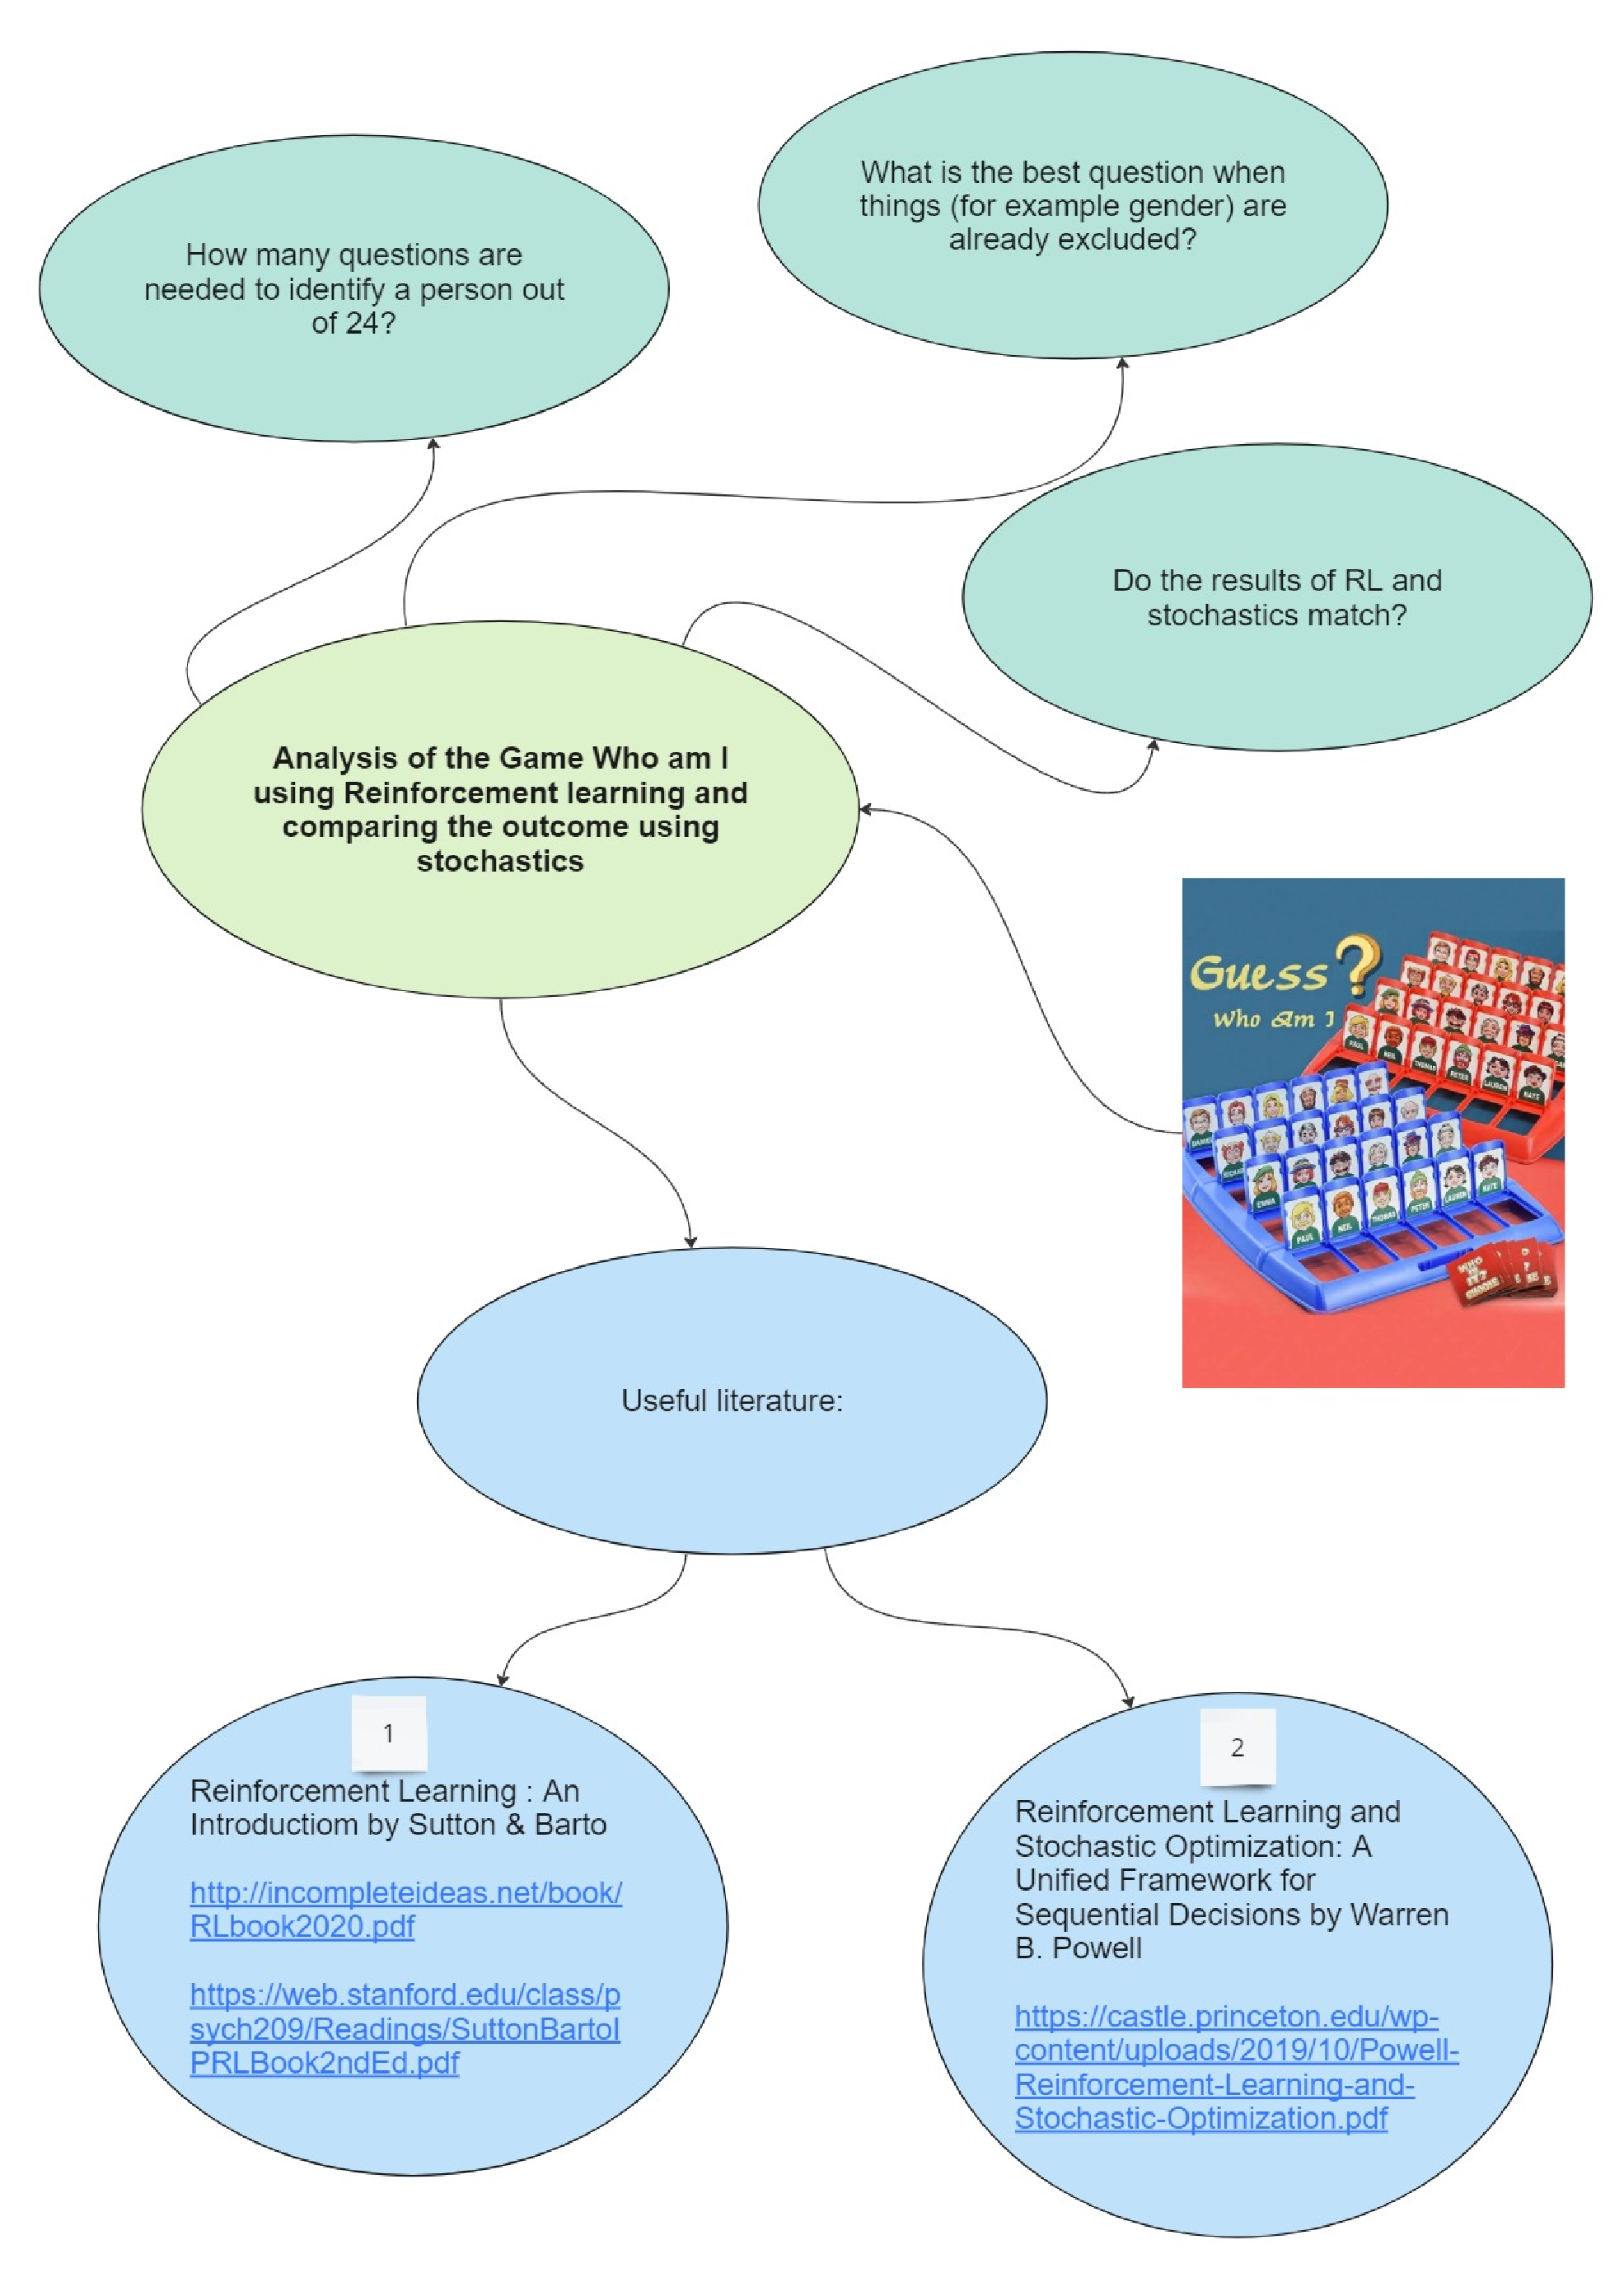
\includegraphics[width=\linewidth]{../pdfs/Mindmap.pdf}
\end{center}

\section{Proposed Literature}

\begin{itemize}
	\item https://www.smithsonianmag.com/science-nature/math-card-game-spot-it-180970873/
	\item https://kraket.nl/en/sector/article/2021-01-04-the-combinatorics-of-sudoku	
	 \item https://lifehacker.com/almost-always-win-the-game-guess-who-with-this-math-bas-1743859796
	\item https://arxiv.org/pdf/1509.03327 (+ Code https://github.com/cerule7/Guess-Who)
	\item https://www.btelligent.com/en/blog/guess-who-for-data-science-enthusiasts/
	\item https://lifebetweensummers.com/guess-who-game-cards-number-sense-and-place-value-activity-for-math-centers/
	\item https://arxiv.org/pdf/1611.03218
\end{itemize}
